\section{Otros objetos}

\subsection{Sin paquetes externos}

\begin{frame}{Imágenes}
  \begin{columns}
    \column{.4\textwidth}
      Incluimos imágenes con el comando \texttt{includegraphics}.

      \espacio

      Indicamos el tamaño con las opciones \texttt{width} y \texttt{height}.
    \column{.6\textwidth}
      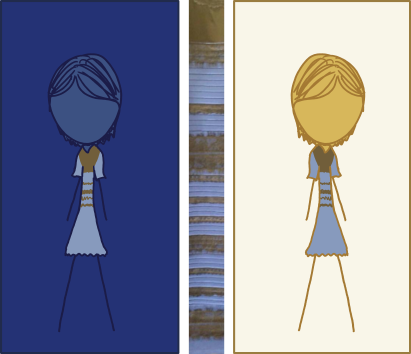
\includegraphics[width=\textwidth]{./img/dress_color.png}
      \\
      \begin{center}
        {\footnotesize \textit{De \href{http://xkcd.com/1492}{xkcd}: Dress colour}.}
      \end{center}
  \end{columns}
\end{frame}

\begin{frame}{Enlaces internos}
  \texttt{hypertarget} y \texttt{hyperlink} nos permiten crear enlaces internos:
  \espacio
  \begin{columns}
    \column{.5\textwidth}
      \pause
      \begin{exampleblock}{Crear enlaces}
        Pulsando \hyperlink{ls}{\color{links}aquí} vamos a la diapositiva anterior. Para
        crear este enlace icluimos:
        \begin{enumerate}
          \item \texttt{\textbackslash {\color{keywords}hypertarget}\{ls\}\{\}} \\
          en la diapositiva anterior.
          \item \texttt{\textbackslash {\color{keywords}hyperlink}\{ls\}\{aquí\}} \\
          en esta diapositiva.
        \end{enumerate}

        Podemos apuntar a un cierto nivel de \textit{overlay}.
      \end{exampleblock}
    \column{.5\textwidth}
      \pause
      \begin{exampleblock}{Botones}
        Podemos crear 3 tipos de botones. Son útiles para añadir enlaces internos:
        \begin{enumerate}
          \item \texttt{beamergotobutton}   \\ \hyperlink{graphs}{\beamergotobutton{Gráficos}}
          \item \texttt{beamerskipbutton}   \\ \hyperlink{end}{\beamerskipbutton{Final}}
          \item \texttt{beamerreturnbutton} \\ \hyperlink{index}{\beamerreturnbutton{Índice}}
        \end{enumerate}
      \end{exampleblock}
  \end{columns}
\end{frame}

\subsection{Con paquetes externos}

\begin{frame}{Listings}
  \hypertarget{ls}{}
  Para incluir código en las diapositivas utilizamos el paquete
  \href{https://www.ctan.org/tex-archive/macros/latex/contrib/listings}{\texttt{listings}}:
  \espacio
  \ejemplo{listing.tex}
  \espacio
  \pause
  \begin{alertblock}{Ajustando \texttt{listings}}
    Debemos incluir la opción \texttt{fragile} a las diapositivas con código.
    Además, debemos \href{http://tex.stackexchange.com/questions/24528}{extender}
    los caracteres para mostrar los que no sean ASCII.
  \end{alertblock}
\end{frame}

\begin{frame}{Gráficos}
\hypertarget{graphs}{}
  \begin{columns}[c]
    \column{.6\textwidth}
      \begin{tikzpicture}
        \begin{axis}[
        ybar stacked,
        bar width=.7cm,
        ytick=\empty,
        symbolic x coords={\beamer,LibreOffice,PowerPoint},
        xtick=data,
        ]
          \addplot[fill=bars] coordinates
          {(\beamer,100) (LibreOffice,9) (PowerPoint,4)};
        \end{axis}
      \end{tikzpicture}

    \column{.4\textwidth}
     Podemos hacer gráficos con \href{https://ctan.org/pkg/pgfplots}{\texttt{pgfplots}}
     (aunque de este paquete se puede hablar tanto como de \beamer).
  \end{columns}
\end{frame}

\begin{frame}{Aún hay más...}
  \hypertarget{end}{}
  \transglitter<1>
  \setbeamercovered{dynamic}
  No he podido cubrir todas las cosas que nos permite hacer \beamer \frownie{}.
  Entre otras cosas, también podemos hacer:
  \espacio
  \begin{description}[<+->]
    \item[Transiciones] Con \texttt{transglitter} obtenemos este efecto.
    \item[Multimedia] Incluir vídeos o sonido con reproductor interno o externo.
    \item[Temporización] Ajustamos el tiempo de una diapositiva con \texttt{transsetduration}.
    \item[Animaciones] No he conseguido que funcionen \frownie{}.
    \item[Cajas] Podemos definir cajas para meter texto.
    \item[Overlays de imágenes] Incluyendo, por ejemplo, dinosaurios.
  \end{description}
  \espacio
  \uncover<5>{
  \begin{beamercolorbox}[shadow=true, rounded=true]{block title}
    Una caja de ejemplo.
  \end{beamercolorbox}
  }

    \alt<7>{%
      \begin{tikzpicture}[remember picture, overlay]
        \node[inner sep=1pt] at (current page.center) {%
            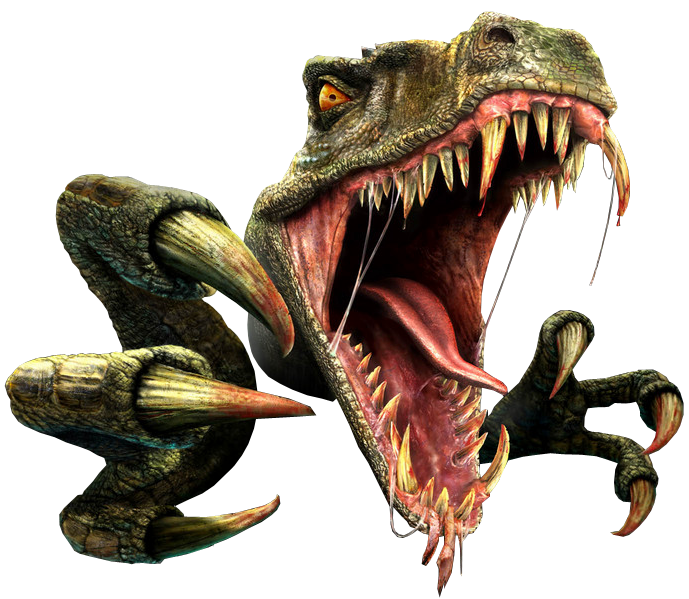
\includegraphics[width=.9\paperwidth,height=.9\paperheight]{./img/dinosaurio.png}%
        };%
      \end{tikzpicture}
    }{\espacio}
\end{frame}
